\documentclass{article}
\usepackage{amsmath, sfmath, multicol, tkz-euclide, array, enumerate, tcolorbox, tabularray}
\renewcommand{\familydefault}{\sfdefault}
\setlength{\parindent}{0cm}
\pagestyle{empty}
\usepackage[left=1in, top=0.5in, right=1in, bottom=0.5in]{geometry}
\tikzset{>=stealth, label style/.append style={font=\footnotesize}}
\tcbset{colback=white}

\newcounter{example}[section]
\newenvironment{example}[1][]{\refstepcounter{example}\par\medskip
   {\color{red}\textbf{Example~\theexample. #1}}}{\medskip}

\begin{document}

\section*{Trigonometry}

\begin{tcolorbox}[colframe=orange!70!white, coltitle=black, title=\textbf{Today I Can}]
\begin{enumerate}
    \item Use trigonometry and inverse trigonometry to find unknown angle measures and side lengths in right triangles.
\end{enumerate}
\end{tcolorbox}
\bigskip 

\begin{minipage}{0.3\textwidth}
\begin{tikzpicture}[scale=0.8]
\tkzDefPoints{0/0/A, 3/0/C, 3/2/B}
\tkzDrawPolygon(A,B,C)
\tkzLabelPoints[left](A)
\tkzLabelPoints[right](B,C)
\tkzMarkRightAngle(B,C,A)
\tkzLabelSegments[right](B,C){$a$}
\tkzLabelSegments[below](A,C){$b$}
\tkzLabelSegments[above left](A,B){$c$}
\end{tikzpicture}
\end{minipage}
\begin{minipage}{0.6\textwidth}
\begin{itemize} \setlength{\itemsep}{15pt}
    \item \textbf{sine} of $\angle A = \sin A = \frac{\text{length of leg opposite }\angle A}{\text{length of hypotenuse}} = \frac{a}{c}$
    
    \item \textbf{cosine} of $\angle A = \cos A = \frac{\text{length of leg adjacent to }\angle A}{\text{length of hypotenuse}} = \frac{b}{c}$

    \item \textbf{tangent} of $\angle A = \tan A = \frac{\text{length of leg opposite }\angle A}{\text{length of leg adjacent to }\angle A} = \frac{a}{b}$
\end{itemize}
\end{minipage}
\smallskip 

\begin{center}
\begin{Large}
$\boxed{\text{S}_{\text{H}}^{\text{O}}  \, \text{C}_{\text{H}}^{\text{A}} \,
\text{T}_{\text{A}}^{\text{O}}}$
\end{Large}
\end{center}

\begin{example}
Given the figure below, find the sine, cosine, and tangent for the indicated angle.
\begin{center}
    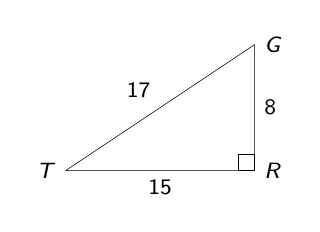
\begin{tikzpicture}[scale=0.8]
    \tkzDefPoints{0/0/T, 3/0/R, 3/2/G}
    \tkzDrawPolygon(T,R,G)
    \tkzLabelPoints[left](T)
    \tkzLabelPoints[right](R,G)
    \tkzMarkRightAngle(G,R,T)
    \tkzLabelSegments[right](G,R){8}
    \tkzLabelSegments[below](T,R){15}
    \tkzLabelSegments[above left](T,G){17}
    \end{tikzpicture}
\end{center}
\begin{multicols}{2}
\begin{enumerate}[(a)]
    \item $\angle T$
    \item $\angle G$
\end{enumerate}
\end{multicols}
\end{example}

\vspace{1.5in}

\subsection*{Finding Missing Side Lengths}
\smallskip 

To find missing side lengths in triangles using trigonometry, you can use
\begin{itemize}
    \item the definition of trig ratios (SOH-CAH-TOA)
    \item your calculator
    \item proportions
\end{itemize}

\newpage 

\begin{example}
Find the value of $w$ to the nearest tenth in each.  \newline\\

\begin{tabular}{p{0.3\linewidth}p{0.3\linewidth}p{0.3\linewidth}}
(a) &   (b) &   (c) \\
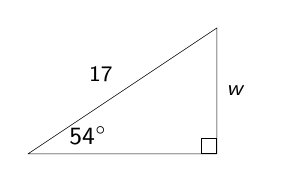
\begin{tikzpicture}[scale=0.8]
\tkzDefPoints{0/0/T, 3/0/R, 3/2/G}
\tkzDrawPolygon(T,R,G)
\tkzMarkRightAngle(G,R,T)
\tkzLabelSegments[right](G,R){$w$}
\tkzLabelAngle[](R,T,G){\small $54^\circ$}
\tkzLabelSegments[above left](T,G){17}
\end{tikzpicture}
&
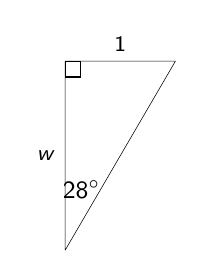
\begin{tikzpicture}[scale=0.8]
\tkzDefPoints{0/0/A, 1.75/0/B, 0/-3/C}
\tkzDrawPolygon(A,B,C)
\tkzMarkRightAngle(B,A,C)
\tkzLabelSegment[left](A,C){$w$}
\tkzLabelSegment[above](A,B){1}
\tkzLabelAngle[](B,C,A){\small $28^\circ$}
\end{tikzpicture}
&
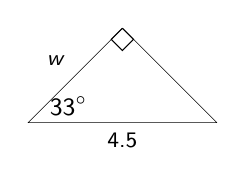
\begin{tikzpicture}[scale=0.8]
\tkzDefPoints{0/0/A, 3/0/B, 1.5/1.5/C}
\tkzDrawPolygon(A,B,C)
\tkzLabelSegment[below](A,B){4.5}
\tkzLabelSegment[above left](A,C){$w$}
\tkzMarkRightAngle(B,C,A)
\tkzLabelAngle[pos=0.7](B,A,C){\small $33^\circ$}
\end{tikzpicture}
\end{tabular}
\end{example}

\vspace{2in}

\subsection*{Finding Missing Angle Measures}
\smallskip 

To find the measures of the angles, use \textbf{inverse} trig ratios:   \newline

$\sin^{-1}$, \qquad  $\cos^{-1}$, \qquad $\tan^{-1}$
\vspace{0.75in}

\begin{example}
Find the measure of the indicated angle to the nearest degree.

\begin{multicols}{3}
\begin{enumerate}[(a)]
    \item $\angle X$
    \item $\angle X$
    \item $\angle Y$
\end{enumerate}
\end{multicols}
\begin{minipage}{0.3\textwidth}
    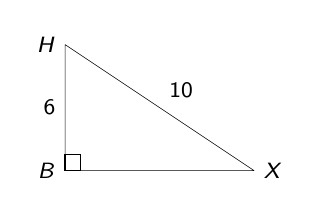
\begin{tikzpicture}[scale=0.8]
    \tkzDefPoints{0/0/B, 3/0/X, 0/2/H}
    \tkzDrawPolygon(B,X,H)
    \tkzLabelPoints[left](B,H)
    \tkzLabelPoints[right](X)
    \tkzLabelSegment[left](H,B){6}
    \tkzLabelSegment[above right](X,H){10}
    \tkzMarkRightAngle(X,B,H)
    \end{tikzpicture}
\end{minipage}
\begin{minipage}{0.3\textwidth}
    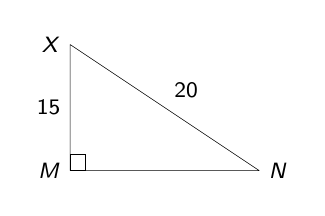
\begin{tikzpicture}[scale=0.8]
    \tkzDefPoints{0/0/M, 3/0/N, 0/2/X}
    \tkzDrawPolygon(X,M,N)
    \tkzLabelPoints[left](X,M)
    \tkzLabelPoints[right](N)
    \tkzLabelSegment[left](X,M){15}
    \tkzLabelSegment[above right](X,N){20}
    \tkzMarkRightAngle(N,M,X)
    \end{tikzpicture}
\end{minipage}
\begin{minipage}{0.3\textwidth}
    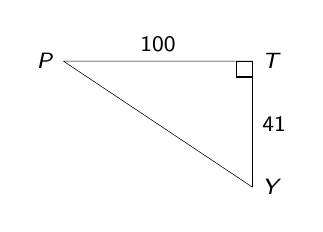
\begin{tikzpicture}[scale=0.8]
    \tkzDefPoints{0/0/P, 3/0/T, 3/-2/Y}
    \tkzDrawPolygon(P,T,Y)
    \tkzLabelPoints[left](P)
    \tkzLabelPoints[right](T,Y)
    \tkzMarkRightAngle(Y,T,P)
    \tkzLabelSegment[above](P,T){100}
    \tkzLabelSegment[right](T,Y){41}
    \end{tikzpicture}
\end{minipage}
\end{example}

\end{document}
